\section{Ovládání}

\subsection*{Procesor}
    Pro samotné fungování a ovládání drona je potřeba procesor, který bude vzdáleně přijímat příkazy a předávat je jednotlivým částem drona. Pro tento úkol jsem zvolil čim ESP-WROOM32 pro jeho nízkou hmotnost, implementovanou podporu Wi-Fi a jeho dvě jádra, která umožňují pruběh více procesů zároveň.
    
\subsection*{Gyroskop}
    Pro automatické vyvažování drona musíme přidat také gyroskop, protože bouhužel námi vyraný procesor jej neobsahuje. Pro projekt nám bude vyhovovat tří-osý gyroskop s akcelerometrem MPU-6050. Tato komponenta je schopna změřit odchylku na třech hlavních osách, podle které upravíme rychlost motorů pro vyrovnání drona. Změřené odchylky si nazveme "ROLL" pro osu x, "PITCH" pro osu y a "YAW" pro osu z.
    
\section{Pohon}

\subsection*{Motory}
    Aby dron byl schopen letu, potřebujeme motory. Nejčastějším provedením je kvadrokoptéra, která má motory čtyři. Vybral jsem motory od BetaFPV, pro jejich nevelkou hmotnost, nízkou cenu a jejich časté použití v levných a lehkých dronech.\cite{motorv1} Výběr byl proveden po konzultaci s poradcem v obchodě FYFT.CZ, který mě obeznámil, že vypočítat přesně kolik motor je schopen unést a předem vědět, který motor vybrat nelze, je to pouze o dobrém odhadu a zkušenostech. Pro správné fungování je potřeba, aby se dva motory na diagonále otáčely stejným směrem a zbylé dva směrem opačným, čímž dosáhneme vynulování otáčení po ose z. Pokud by se všechny motory otáčely stejným směrem, dron by nám rotoval.
    
\newpage

\subsection*{L293D}
    Pro ovládání motoru využívám dva drivery L293D, kde každý ovládá dva motory. Tento driver funguje na principu dvou AND hradel, kde jedno je stále na hodnotě LOW a druhé má na vstupu hodnotu HIGH a PWM signál poskytnutý ESP. PWM signálem jsme schopni omezit rychlost otáček a snížit tím rychlost stoupání.
    
\section{Napájení}

\subsection*{Baterie}
    Nejvhodnější baterií pro takovýto projekt je typ Li-Pol, protože jsou lehké, s velkou kapacitou a mohou se nabíjet narozdíl od jiných baterií. S limitním napětím našich motorů hodnoceným na 5V potřebujeme dvojčlánkovou Li-Pol baterii s napětím 7,4V, které pomocí součástek v další části snížíme na požadovaných 5V. Po spočítání spotřeby motorů a čipů jsme se rozhodl pro baterii KAVAN Li-Po 860mAh/7,4V, která by měla vydržet při nejvyšší zátěži přibližně patnáct minut.
    
\subsection*{Regulace}
    Náš dron potřebuje dvě napětí - 3,3V pro ESP a MPU a 5V pro L293D a motory. V prvním provedení jsem tohoto dosáhl za pomocí dvou lineárních regulátorů napětí LM7805C zapojených do serie. Tento postup bohužel prakticky nefungoval, i když jsme dosáhli požadovaných napětí, první regulátor se ihned přehřál na kritickou teplotu a vypínal se. Řešením bylo vyměnit první regulátor z 7,4V na 5V za Step-Down converter, který je sice větší a těžší, ale efektivnější a nepřehřívá se.
    
    \begin{figure}[h]
        \centering
        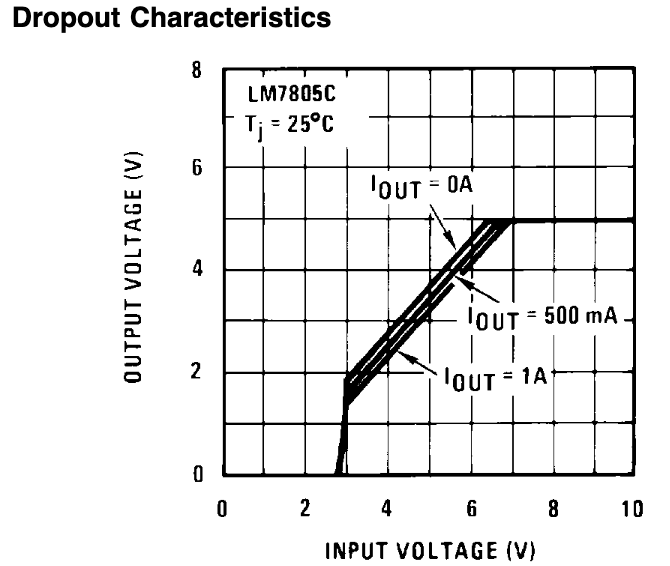
\includegraphics[scale=0.7]{img/regulartor.png}
        \caption{Výstupní napětí v závislosti na vstupním u regulátoru LM7805C\cite{LM7805C}}
    \end{figure}


